\documentclass[a4paper, 12pt]{article}
\usepackage[usenames,dvipsnames,svgnames,table]{xcolor}
\usepackage[T1]{fontenc}
\usepackage{times}
\usepackage[utf8]{inputenc}
\usepackage{wallpaper}
\usepackage[absolute]{textpos}
\usepackage[top=2cm, bottom=2.5cm, left=3cm, right=3cm]{geometry}


\newsavebox{\mybox}
\newlength{\mydepth}
\newlength{\myheight}
\newenvironment{sidebar}
{\begin{lrbox}{\mybox}\begin{minipage}{\textwidth}}
{\end{minipage}\end{lrbox}
 \settodepth{\mydepth}{\usebox{\mybox}}
 \settoheight{\myheight}{\usebox{\mybox}}
 \addtolength{\myheight}{\mydepth}
 \noindent\makebox[0pt]{\hspace{-20pt}\rule[-\mydepth]{1pt}{\myheight}}
 \usebox{\mybox}}

\newcommand\BackgroundPic{
    \put(-2,-3){
    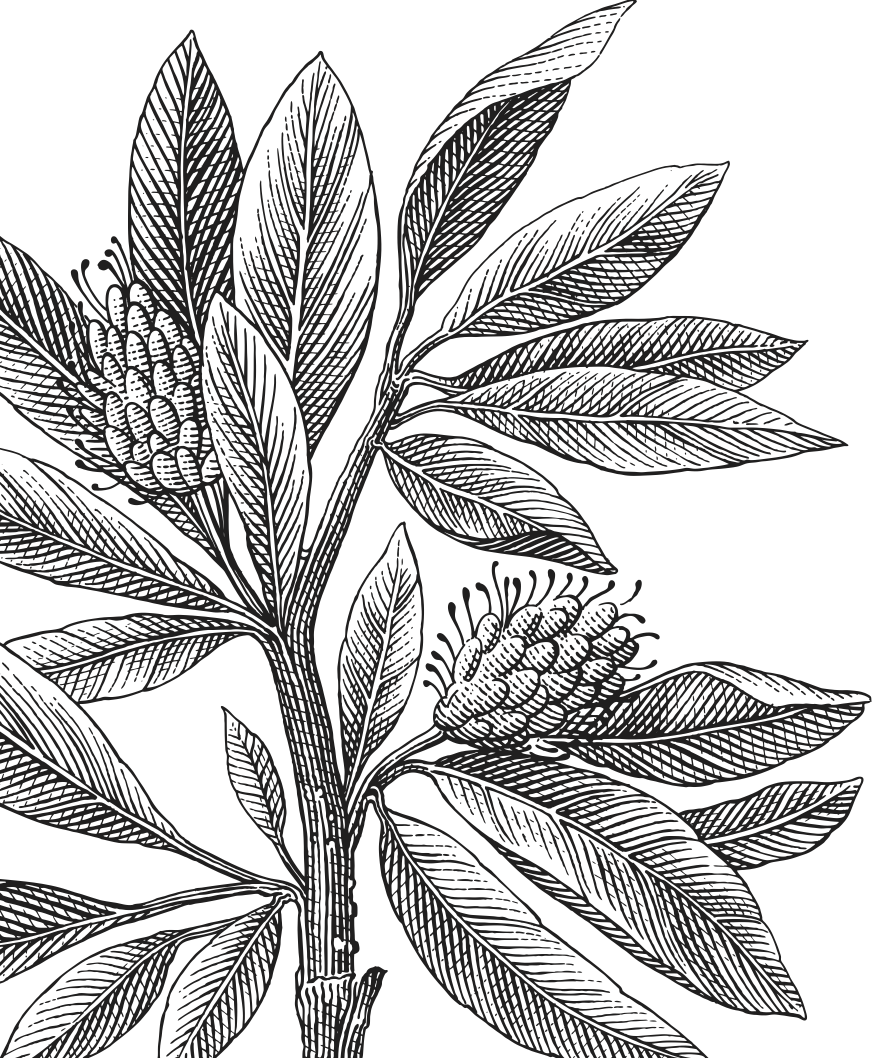
\includegraphics[keepaspectratio,scale=0.3]{../lnu_etch.png} 
    }
}
\newcommand\BackgroundPicLogo{
    \put(30,740){
	
\includegraphics[keepaspectratio,scale=0.10]{../logo.png}     
    }
}

\title{	
\vspace{-8cm}
\begin{sidebar}
    \vspace{5cm}
    \normalfont \normalsize
    \Huge Report \\
    \vspace{-1.3cm}
\end{sidebar}
\vspace{3cm}
\begin{flushleft}
    \huge Test Report\\  
\end{flushleft}
\null
\vfill
\begin{textblock}{6}(10,13)
\begin{flushright}
\begin{minipage}{\textwidth}
\begin{flushleft} \large
	\emph{Author:} \\ Caroline Nilsson \textit{(cn222nd)} \\ Daniel Alm Grundström \textit{(dg222dw)} \\
	%\emph{Handledare:} \\ 
	\emph{Term:} HT 2017\\ 
	\emph{Course:} 2DV610 - Software Testing\\
\end{flushleft}
\end{minipage}
\end{flushright}
\end{textblock}
}
\date{\today} 

\begin{document}

\pagenumbering{gobble}
\newgeometry{left=5cm}
\AddToShipoutPicture*{\BackgroundPic}
\AddToShipoutPicture*{\BackgroundPicLogo}
\maketitle
\restoregeometry
\clearpage

\pagenumbering{gobble}

\tableofcontents
\newpage
\pagenumbering{arabic}

\section{Traceability Matrix}

\begin{tabular}{|c|c|c|c|c|c|c|}
\hline
\multicolumn{7}{|c|}{Requirement Matrix} \\ \hline
Requirement	& Reqs			& Req. 1		& 	Req. 2		&  Req. 3		& Req. 5 		& Req. 5	\\ 
Identifiers		& Tested		&					&	UC3			& 					&	UC1			& UC2		\\ \hline
Test Cases	&					&					&					&	5				&	3				&	2			\\ \hline
1.1				& 					&					&					&	X				&	X				&				\\ \hline
1.2				& 					&					&					&	X				&	X				&				\\ \hline
1.3 				& 					&					&					&	X				&	X				&				\\ \hline
2.1				&					& 					& 					&	X				&					&	X			\\ \hline
2.2				&					&					& 					&	X				&					&	X			\\ \hline

\end{tabular}



\section{Test Cases - Result}

\newpage


\end{document}
